\documentclass[utf8, a4paper, 12 pt]{article}
\usepackage{graphicx, float}
\usepackage{fourier}
\usepackage[french]{babel}
\usepackage[T1]{fontenc}
\usepackage[utf8]{inputenc}
\usepackage{enumitem, pifont}
\usepackage{amsmath, amsfonts,amssymb}                                                                                                                                                                                                                                                                                                                                                                                                                                                                                                                                                                                                                                                                                                                                                                                                                                                                                                                                                                                                                                                                                                                                                                                                                                                                                                                                                                                                                                                                                                                                                                                                                                                                                                                                                                                                                                                                                                                                                                                                                                                                                                                                                                                                                                                                                                                                                                                                     

\title{\LARGE \textbf{SURFACES ET SOLIDES}}
\author{MATH\'EMATHIQUES 6P}
\date{\today}
\setlist[itemize, 1]{label ={\ding{248}}, itemsep = \baselineskip}



\begin{document}

    \large
    \everymath{\displaystyle}
    \begin{titlepage}  
        \maketitle
    \end{titlepage} 
    \setcounter{page}{2}

    \section{Mesurer une surface}

        \subsection{notion d'aire}
            La mesure d'une surface s'appelle une \emph{aire} même si,
            dans le langage courant, 
            on utilise également le mot \emph{surface}.\\%\vspace{1\baselineskip}
            L'aire correspond à un nombre de carrés qu'on peut découper dans cette surface.\\\\
            \emph{Exercice :}
            \begin{itemize}
                \item calcule l'aire de la classe en \og découpant \fg{} sa surface en carrés de 1m de côté
            \end{itemize} 

        \subsection{unités d'aires}
        
            L'unité d'aire utilisée correspond au carré que l'on utilise pour calculer(compter) l'aire.\\
            Les unités les plus utilisées sont :
            \begin{itemize}
                \item $m^2$
                \item $cm^2 \quad 1m^2 = 10 000 cm^2$
                \item $mm^2 \quad 1cm^2 = 100 mm^2$
                \item $ha (hectare) \quad 1 ha = 10\,000 m^2$
                \item $a (are) \quad 1 a = 100 m^2$
                \item $ca (centiare) \quad 1 ca = 1 m^2$ 
            \end{itemize} 
            \vspace{1\baselineskip}
            
            \emph{Exercices}:
            Calcule l'aire dans l'unité demandée : 
            \begin{enumerate}[label = \Alph*) ]
                \item $5 m^2 \quad en\; mm^2$
                \item $3 ha~2 a~5 ca \quad en \; m^2$
                \item $1500 cm^2 \quad en \; m^2$
            \end{enumerate}

        \subsection{Formules d'aires}
        L'aire de certaines surfaces particulières se calculent à l'aide de formules:
            \begin{figure}[H]
                \centering
                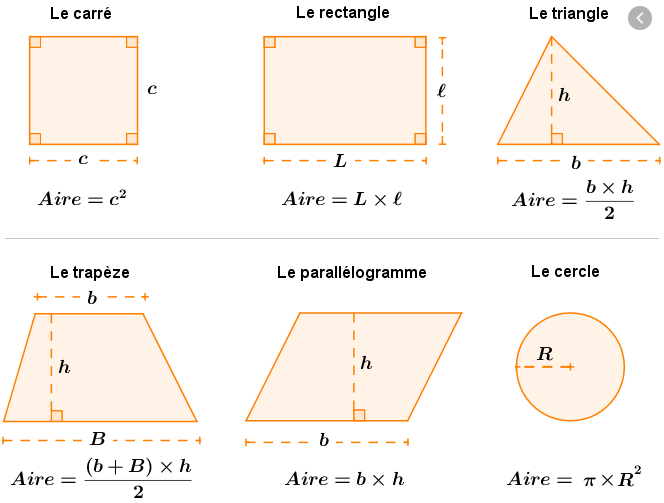
\includegraphics[width=0.9\linewidth]{img/formuleAires.PNG}
                \caption{Aires de quelques surfaces}
            \end{figure}

        \subsection{Exercice : Aire d'un appartement}
            Calcule l'aire de chaque pièce de l'appartement 1 (figure 2), puis son aire totale.
            Si certaines mesures sont manquantes, évalue-les.
            \begin{figure}[H]
                \centering
                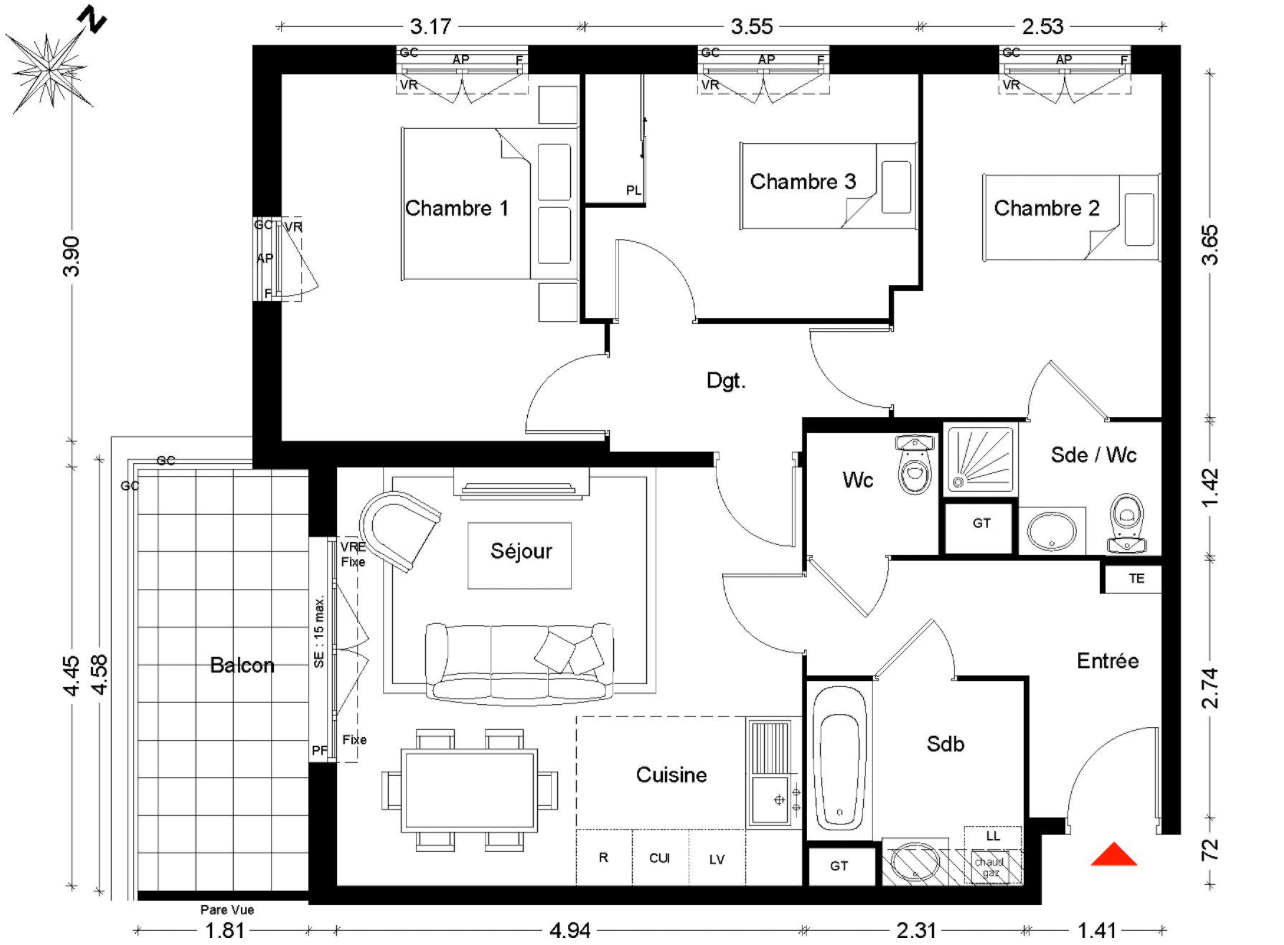
\includegraphics[width=1\linewidth]{img/appartement1.PNG}
                \caption{Plan de l'appartement 1}
            \end{figure}

\end{document}
